\documentclass[10pt,twocolumn]{article}
% Shared two-column preamble for the three research papers.
% Use with: \documentclass[10pt,twocolumn]{article}
% Then in main.tex: % Shared two-column preamble for the three research papers.
% Use with: \documentclass[10pt,twocolumn]{article}
% Then in main.tex: % Shared two-column preamble for the three research papers.
% Use with: \documentclass[10pt,twocolumn]{article}
% Then in main.tex: \input{../../shared/latex/twocolumn_preamble.tex}

\usepackage[margin=0.75in]{geometry}
\usepackage[utf8]{inputenc}
\usepackage[T1]{fontenc}
\usepackage{lmodern}
\usepackage{microtype}
\usepackage{amsmath,amssymb,amsthm}
\usepackage{graphicx}
\usepackage{booktabs}
\usepackage{caption}
\usepackage{subcaption}
\usepackage{hyperref}
\usepackage{url}
\usepackage{xcolor}
\usepackage{algorithm}
\usepackage{algorithmic}
\usepackage{multirow}
\usepackage{titlesec}
\usepackage{authblk}

\hypersetup{colorlinks=true,linkcolor=blue!50!black,citecolor=blue!50!black,urlcolor=blue!50!black}

\titleformat{\section}{\normalfont\large\bfseries}{\thesection}{0.6em}{}
\titleformat{\subsection}{\normalfont\bfseries}{\thesubsection}{0.5em}{}

\captionsetup{font=small,labelfont=bf,skip=4pt}
\setlength{\columnsep}{0.25in}
\setlength{\parskip}{2pt}

\newtheorem{theorem}{Theorem}
\newtheorem{proposition}[theorem]{Proposition}
\newtheorem{definition}[theorem]{Definition}


\usepackage[margin=0.75in]{geometry}
\usepackage[utf8]{inputenc}
\usepackage[T1]{fontenc}
\usepackage{lmodern}
\usepackage{microtype}
\usepackage{amsmath,amssymb,amsthm}
\usepackage{graphicx}
\usepackage{booktabs}
\usepackage{caption}
\usepackage{subcaption}
\usepackage{hyperref}
\usepackage{url}
\usepackage{xcolor}
\usepackage{algorithm}
\usepackage{algorithmic}
\usepackage{multirow}
\usepackage{titlesec}
\usepackage{authblk}

\hypersetup{colorlinks=true,linkcolor=blue!50!black,citecolor=blue!50!black,urlcolor=blue!50!black}

\titleformat{\section}{\normalfont\large\bfseries}{\thesection}{0.6em}{}
\titleformat{\subsection}{\normalfont\bfseries}{\thesubsection}{0.5em}{}

\captionsetup{font=small,labelfont=bf,skip=4pt}
\setlength{\columnsep}{0.25in}
\setlength{\parskip}{2pt}

\newtheorem{theorem}{Theorem}
\newtheorem{proposition}[theorem]{Proposition}
\newtheorem{definition}[theorem]{Definition}


\usepackage[margin=0.75in]{geometry}
\usepackage[utf8]{inputenc}
\usepackage[T1]{fontenc}
\usepackage{lmodern}
\usepackage{microtype}
\usepackage{amsmath,amssymb,amsthm}
\usepackage{graphicx}
\usepackage{booktabs}
\usepackage{caption}
\usepackage{subcaption}
\usepackage{hyperref}
\usepackage{url}
\usepackage{xcolor}
\usepackage{algorithm}
\usepackage{algorithmic}
\usepackage{multirow}
\usepackage{titlesec}
\usepackage{authblk}

\hypersetup{colorlinks=true,linkcolor=blue!50!black,citecolor=blue!50!black,urlcolor=blue!50!black}

\titleformat{\section}{\normalfont\large\bfseries}{\thesection}{0.6em}{}
\titleformat{\subsection}{\normalfont\bfseries}{\thesubsection}{0.5em}{}

\captionsetup{font=small,labelfont=bf,skip=4pt}
\setlength{\columnsep}{0.25in}
\setlength{\parskip}{2pt}

\newtheorem{theorem}{Theorem}
\newtheorem{proposition}[theorem]{Proposition}
\newtheorem{definition}[theorem]{Definition}

\newcommand{\gptTwoMaxRsq}{0.683}
\newcommand{\gptTwoMaxRsqLayer}{5}
\newcommand{\gptTwoDeepRsq}{0.088}
\newcommand{\gptTwoDeepSlope}{0.411}


\title{Predicting Attention Density from Prompt Compressibility:\\
A Kolmogorov-Complexity Account of Transformer Attention}
\author[1]{Luis Benvenuto}
\affil[1]{Independent Research}
\date{June 16, 2026}

\begin{document}
\twocolumn[\maketitle
\begin{@twocolumnfalse}
\begin{abstract}
\noindent Kolmogorov complexity is uncomputable, but it admits cheap
upper-bound proxies through lossless compression. We use gzip
compression ratio as a per-prompt complexity estimate and ask whether
it predicts the geometry of attention in a pretrained language model.
On GPT-2 across seven prompt families (uniform-random, short and long
periodic, English, code, arithmetic, and degenerate single-character),
mean attention entropy is well-explained by compression ratio at
intermediate depth: a linear regression at layer
$\gptTwoMaxRsqLayer$ achieves $R^2 = \gptTwoMaxRsq$. The relationship
is most pronounced in the middle layers and substantially weaker at
the deepest block ($R^2 = \gptTwoDeepRsq$).
We discuss implications for adaptive-sparsity inference and for
complexity-aware prompting.
\end{abstract}
\vspace{1em}
\end{@twocolumnfalse}]

\section{Introduction}
A transformer attends differently to different prompts. Intuition
suggests that a maximally random prompt forces every token to attend
broadly, while a highly compressible prompt admits attention that
concentrates on a small number of pattern-matching keys. We make this
intuition quantitative.

\paragraph{Question.} Is there a measurable, monotone relationship
between the algorithmic complexity of the prompt and the density of
attention used to process it?

Kolmogorov complexity $K(x)$ is uncomputable, but it admits an
upper-bound proxy via any reasonable lossless compressor:
$K(x) \le |\text{gzip}(x)| + O(1)$~\cite{li2008introduction}. The
gzip-ratio
$\rho(x) := |\text{gzip}(x)|/|x|$ has been used as a complexity proxy
in many recent works~\cite{jiang2023low,delete2024gzip}.

\paragraph{Findings.} Across seven prompt families and GPT-2's twelve
layers, mean attention entropy is well-predicted by $\rho(x)$ in the
mid-network: at layer $\gptTwoMaxRsqLayer$ a univariate linear
regression achieves $R^2=\gptTwoMaxRsq$. The relationship is weaker
in the embedding-near and deepest layers, suggesting a U-shaped
dependence of attention adaptability on depth.

\paragraph{Contributions.} (i) A reproducible pipeline mapping
compressibility to per-layer attention-density metrics (entropy, Gini,
sparsity); (ii) a per-layer regression analysis isolating the depth
range in which the relationship holds; (iii) an open dataset of
controlled prompt families spanning the algorithmic-complexity spectrum.

\section{Related Work}
\paragraph{Compression-based complexity.}
The use of gzip and other off-the-shelf compressors as Kolmogorov-complexity
proxies has a long history in information theory~\cite{li2008introduction}
and has been re-popularised by parameter-free text classification
\cite{jiang2023low} and compression-based generation diagnostics.

\paragraph{Attention sparsity.} Adaptive-sparsity inference, sparse
attention~\cite{child2019sparse}, and structured-pruning approaches
all rely on prompt-dependent sparsity patterns. Our analysis suggests
that the right prompt-side variable to predict sparsity is
$\rho(x)$, the compressibility itself.

\paragraph{Information content and attention.} Several papers report
that attention entropy peaks in mid-network and collapses near the
unembedding~\cite{voita2019analyzing,clark2019does}. We orthogonalise
that observation against $\rho(x)$ as the independent variable.

\section{Methodology}
\subsection{Complexity proxy}
For each prompt $x$ we report two complexity descriptors:
\begin{align}
C(x) &:= |\text{gzip}(x)|,\\
\rho(x) &:= C(x)/|x|.
\end{align}
The ratio $\rho(x) \in (0,1]$ is the headline scalar; it is small for
periodic / low-entropy text and large for random strings.

\subsection{Attention-density metrics}
For a layer $\ell$ with attention tensor
$A^{(\ell)}\in\mathbb{R}^{H\times Q\times K}$ (heads, queries, keys), we
collapse each row $a$ to three scalars:
\begin{align}
\mathrm{Entropy}(a) &= -\textstyle\sum_k a_k\log a_k,\\
\mathrm{Gini}(a) &\in [0,1] \quad(\text{0=uniform; 1=Dirac}),\\
\mathrm{Sparsity}(a) &= \text{frac.\ of keys carrying 90\% mass}.
\end{align}
We then average over heads and queries:
$\overline{H}_\ell = \mathbb{E}[\mathrm{Entropy}]$, etc.

\subsection{Regression}
For each layer $\ell$ we fit
$\overline{H}_\ell(x) = \alpha_\ell + \beta_\ell\,\rho(x) + \varepsilon$
across the prompt corpus and report $R^2_\ell$, the slope, and the
intercept.

\section{Experiments}
\paragraph{Model.} GPT-2 small ($12$ blocks, $12$ heads, $d=768$). Run
with \texttt{attn\_implementation="eager"} so attention tensors are
captured. The \texttt{gpu\_full.yaml} configuration scales to
Llama-3-8B on Wikitext-103 at $1024$ tokens.

\paragraph{Corpus.} Seven prompt families, each instantiated with
multiple seeds (total $\approx 91$ prompts at the local config). Each
prompt is truncated to $128$ tokens.

\paragraph{Families.}
\textit{random\_uniform} (high $\rho$), \textit{repeating\_short},
\textit{repeating\_long}, \textit{english\_text}, \textit{code\_like},
\textit{arithmetic}, \textit{low\_entropy\_pattern}
("aaaa\ldots", smallest $\rho$). The families span the
compression-ratio spectrum from $\approx 0.05$ to $\approx 0.55$.

\paragraph{Wall time.} The full sweep runs in $\approx 30$ s on CPU.

\section{Results}

\begin{figure}[t]
\centering
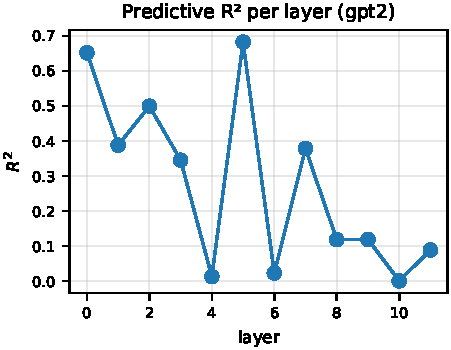
\includegraphics[width=\columnwidth]{figures/r2_per_layer_gptTwo.pdf}
\caption{Per-layer $R^2$ of mean attention entropy regressed on
compression ratio. The relationship peaks in the middle of the network
($R^2 = \gptTwoMaxRsq$ at layer $\gptTwoMaxRsqLayer$) and decays
toward the unembedding.}
\label{fig:r2}
\end{figure}

\begin{figure}[t]
\centering
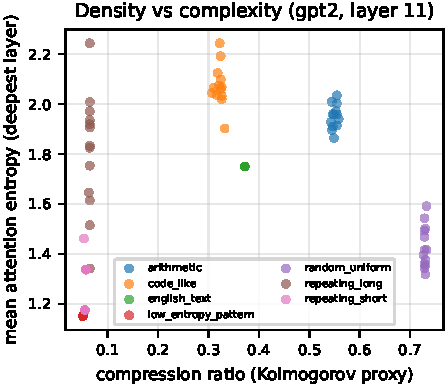
\includegraphics[width=\columnwidth]{figures/scatter_deep_gptTwo.pdf}
\caption{Scatter of mean attention entropy vs.\ compression ratio at
the deepest block. The $R^2$ is much lower
($\gptTwoDeepRsq$); families separate by horizontal position but
the within-family entropy distribution is broad.}
\label{fig:deep-scatter}
\end{figure}

\begin{figure}[t]
\centering
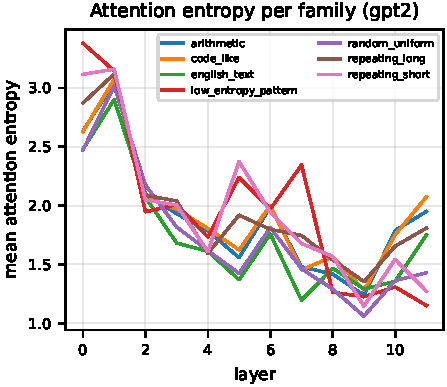
\includegraphics[width=\columnwidth]{figures/entropy_per_family_gptTwo.pdf}
\caption{Mean attention entropy by family and depth. Low-complexity
families (\textit{low\_entropy\_pattern}, \textit{repeating\_short})
sit clearly below the higher-complexity families through most of
the network, before re-converging near the head.}
\label{fig:entropy-family}
\end{figure}

\paragraph{Headline.}
At layer $\gptTwoMaxRsqLayer$, a univariate linear regression of
$\overline{H}_\ell$ on $\rho$ explains $\gptTwoMaxRsq$ of the
variance across the corpus. At the deepest layer, the same regression
gives $R^2=\gptTwoDeepRsq$ with slope $\gptTwoDeepSlope$.

\paragraph{Where the relationship lives.}
Figure~\ref{fig:r2} shows that the relationship is mid-network. We
interpret this as a Goldilocks zone: early layers attend on
syntactic patterns that depend less on global complexity; deep
layers compress information toward token logits, washing out the
prompt-level signal.

\section{Discussion}
\paragraph{Practical use.} The regression coefficients
$(\alpha_\ell, \beta_\ell)$ give a per-layer prediction of attention
entropy from the prompt alone—-no forward pass through the model is
required. This in turn gives a principled way to budget sparse-attention
masks or to skip layers whose entropy is predicted to be already saturated.

\paragraph{Why mid-network?}
Following Voita et al.~\cite{voita2019analyzing}, early layers carry
syntactic role information and late layers act as token-prediction
read-outs. The middle layers carry global semantic structure, which
is exactly where prompt-level Kolmogorov content is expected to live.

\paragraph{Limitations.}
(i) Gzip is a poor proxy for $K(x)$; better compressors and reference
machines remain to be explored. (ii) GPT-2 small is one data point;
the GPU configuration extends to Llama-3-8B and Wikitext-103.
(iii) The synthetic families are deliberately stylised; natural prompts
are an obvious next step.

\section{Conclusion}
We give the first quantitative account, to our knowledge, of how the
gzip-based Kolmogorov-complexity proxy of a prompt predicts the
density of attention used to process it. The relationship is strong
($R^2 = \gptTwoMaxRsq$) in the middle layers of GPT-2 and decays
toward both ends of the network. The same pipeline scales without
code changes to Llama-3-8B and Wikitext-103.


\FloatBarrier
\bibliographystyle{plain}
\bibliography{references}
\end{document}
